\documentclass[10pt,twocolumn]{article}

\usepackage[T1]{fontenc}
\usepackage[utf8]{inputenc}
\usepackage[margin=0.75in, top=1.0in, bottom=0.9in]{geometry}
\IfFileExists{binhex.tex}{\usepackage{newtxtext}}{}
\usepackage{amsmath}
\usepackage{amssymb}
\IfFileExists{binhex.tex}{\usepackage{newtxmath}}{}
\usepackage[expansion=false]{microtype}
\usepackage[numbers,sort&compress]{natbib}
\usepackage[dvipsnames]{xcolor}
\usepackage[colorlinks=true, linkcolor=MidnightBlue, citecolor=MidnightBlue,
            urlcolor=MidnightBlue, bookmarks=false]{hyperref}
\usepackage{booktabs}
\usepackage{graphicx}
\usepackage{placeins}
\graphicspath{{results/figures/paper/}{results/figures/exploratory/}{../../results/figures/paper/}{../../results/figures/exploratory/}}
\usepackage{algorithm}
\usepackage{algpseudocode}
\usepackage[small, labelfont=bf, font=small, skip=4pt]{caption}
\usepackage{titlesec}
\usepackage{enumitem}
\setlist{nosep, leftmargin=1.2em}

% ---------- column / paragraph spacing ----------
\setlength{\columnsep}{0.25in}
\setlength{\parindent}{1em}
\setlength{\parskip}{0pt}

% ---------- section headings (clean NeurIPS/ICML style) ----------
\titleformat{\section}
  {\normalfont\large\bfseries}
  {\thesection}{0.6em}{}
\titleformat{\subsection}
  {\normalfont\normalsize\bfseries}
  {\thesubsection}{0.5em}{}
\titleformat{\subsubsection}[runin]
  {\normalfont\normalsize\bfseries}
  {\thesubsubsection}{0.5em}{}[.\hspace{0.3em}]
\titlespacing*{\section}    {0pt}{10pt plus 2pt minus 1pt}{4pt}
\titlespacing*{\subsection} {0pt}{8pt plus 1pt}{3pt}

% ---------- clean page style (no header rules) ----------
\pagestyle{plain}

\begin{document}

\twocolumn[{%
\begin{center}
\vspace*{-0.3in}
  {\LARGE\bfseries When More Observation Hurts:\\[3pt]
  Redundancy and Robust Clarification\\[1pt]
  in Ask-or-Act Under Instruction Ambiguity}\\[12pt]
  {\large Zhu Yufan}\\[4pt]
  {\small National University of Singapore \quad\textbar\quad CS6208 Final Report}\\[2pt]
  {\small\texttt{A0238993J} \quad\textbar\quad April 10, 2026}
\end{center}
\vspace{12pt}
\centerline{\parbox{0.92\textwidth}{\small
\textbf{Abstract.}\enspace
A cooperative assistant can infer a principal's goal by passively observing actions or actively asking costly questions.
To our knowledge, no prior benchmark controls both channels simultaneously; we build one and use it to study how passive and active evidence interact under a shared success--cost objective.
Three findings emerge from 19{,}800 episodes across six policies.
First, the channels are used sub-additively in this setting, with an interaction of $I{=}{-}26{\pm}3$\,pp at $K{=}3$, suggesting that a cost-aware policy largely extracts overlapping information from each source.
Second, in our benchmark assistability is non-monotonic in principal rationality: NeverAsk success falls from $92\%$ to $84\%$ as $\beta$ rises from 8 to 16 at $K{=}3$, because extreme rationality collapses action diversity and hides intent.
Third, under model mismatch, forced passive observation hurts more than in the matched case ($-2.2$\,pp/step vs.\ $-0.8$\,pp), and decision-layer fixes do not recover this loss; surprise-tempered posterior updates recover $+1$--$+5$\,pp under mismatch with no harm when the model is correct.
}}
\vspace{14pt}
}]

\section{Introduction}

A central challenge in cooperative assistance is deciding when a helper should ask for clarification rather than act.
Acting immediately risks committing to the wrong goal, whereas asking too often wastes time and may frustrate the principal.
The trade-off depends on the informativeness of available questions, the cost of a wrong action, and what the principal's behaviour already reveals.

We study this question by constructing an attribute-structured, post-parsing clarification benchmark in which the candidate goal set is known, question semantics are fixed, and the principal model is given.
The benchmark's value is controlled diagnosis, not ecological realism.
It includes a cooperative principal whose actions are observable for passive inference via inverse planning, and a question bank the assistant may use at explicit cost for active clarification.
The contributions are threefold, comprising a reproducible two-room gridworld with templated instruction ambiguity and a Boltzmann principal model, a systematic comparison of six ask-or-act policies across 19{,}800 episodes, and an empirical characterisation of how the two channels interact.
Our contribution is not a new ask policy, but, to our knowledge, the first controlled characterisation of how the value of active clarification changes as passive action evidence weakens, with the empirical success--question-cost frontier shifting substantially with principal rationality.

\textbf{Why a controlled benchmark?}
Prior work on inverse planning and clarification studies each channel in isolation, as reviewed in the Related Work section below.
To our knowledge, no prior benchmark combines both under controlled ambiguity sweeps, so it has not been possible to measure how the two sources of evidence interact.
Our benchmark is designed to fill exactly this gap.

\textbf{Three Takeaways.}
First, the channels are used \emph{sub-additively}, with $I{=}{-}26$\,pp at $K{=}3$, meaning AskOrAct extracts overlapping information and clarification matters most when passive inference is structurally weak.
Second, assistability is \emph{non-monotonic} in $\beta$, as extreme rationality collapses action diversity and hides intent, causing NeverAsk success to fall at high $\beta$.
Third, under model mismatch, forced observation costs $-2.2$\,pp/step, which is $2.8\times$ the matched rate, explaining why passive-aware decision-layer heuristics fail.
The benchmark is intended as a reusable testbed for future ask-or-act methods.

\section{Related Work}
\label{sec:related}

Inverse planning infers goals from behaviour~\cite{baker2009,ramirez2010plan}. CIRL~\cite{hadfield2016cirl} formalises cooperative teams, and CLIPS~\cite{tan2024clips} adds language evidence, but none of these provides an ask-or-act decision.
Shared autonomy~\cite{javdani2015shared} and HRI clarification~\cite{tellex2014asking,cakmak2012designing} study one channel at a time.
Goal recognition design~\cite{keren2014grd,dragan2013legibility} and PAGR~\cite{zhang2025pagr} target recognition, not task completion with costly typed questions.
ATD~\cite{kobalczyk2025active}, SAGE~\cite{suri2025structured}, and Grand et al.~\cite{grand2026shoot} study clarification without observing principal actions, precluding measurement of channel interaction.
Our benchmark is the first to control both channels simultaneously under a shared success--cost objective.

\section{Method}

\subsection{Environment}

We use a $9{\times}9$ two-room gridworld with $M{=}6$ object instances per episode. The cooperative setup is illustrated in Figure~\ref{fig:setup_overview}.
Room~0 and Room~1 are separated by a mid-wall with a single doorway.
Each episode samples 6 objects from types $\{\text{key}, \text{gem}, \text{coin}\}$ and colours $\{\text{red}, \text{blue}, \text{green}\}$. Exactly $K$ of them match the ambiguous instruction and serve as candidate goals, while the remaining $M{-}K$ are distractors.

A principal has a hidden goal object.
An instruction template maps the goal to a surface form shared by $K$ candidate goals (ambiguity level $K$).
The principal takes approximately rational actions towards its goal, sampled from a Boltzmann policy with rationality $\beta$ and $\varepsilon$-greedy noise:
$\pi_{\beta,\varepsilon}(a \mid s, g) = (1{-}\varepsilon)\,\mathrm{softmax}_\beta\bigl(V(s,\cdot,g)\bigr)_a + \varepsilon/|A|$,
where $V(s,a,g) = -d^*(\mathrm{succ}(s,a),\, g)$ is the negated shortest-path distance from the successor of $a$ to $g$.

The assistant observes the state, instruction, and all principal actions, but not the true goal.
An episode ends when the assistant picks an object, which counts as success if correct, or when the step budget $T_{\max}{=}200$ is exhausted.
The question bank $\mathcal{Q}$ contains three types of questions addressing the goal's colour, room, and object type, each with a factual answer drawn from a per-type noisy channel.
When the assistant decides to ask, it remains at its current position. When it decides to act, it takes one step toward the MAP-goal object via A* navigation and then re-evaluates.

\begin{figure*}[t]
  \centering
  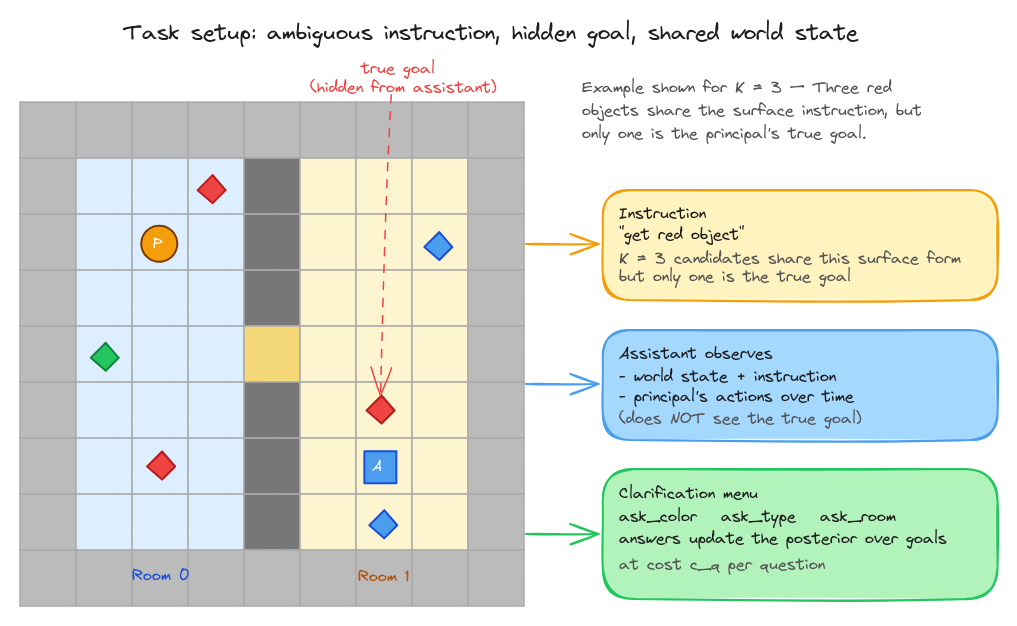
\includegraphics[width=0.7\textwidth]{setup_overview.png}
  \caption{Task setup for $K{=}3$: gridworld and the assistant's three information channels.}
  \label{fig:setup_overview}
\end{figure*}

Full hyperparameters are in Appendix~\ref{app:episode_gen}, Table~\ref{tab:setup}.

\subsection{Bayesian Posterior}

The assistant maintains a posterior $b_t(g)$ over candidate goals, initialised uniformly, and updated at each step via Bayes' rule using the Boltzmann action likelihood for passive observations and a noisy answer channel for active questions. Full update equations are in Appendix~\ref{app:derivation}.

\subsection{Ask-or-Act Policy}
\label{sec:method_askoract}

\textit{AskOrAct} uses a Bayes-risk ask gate to decide \emph{whether} to ask, paired with a separate MAP$+$A* controller for motion execution.
The ask gate compares the expected surrogate team cost, defined as navigation steps plus per-question penalty $c_q$, of asking versus acting under the current posterior $b_t$.
The policy is not a unified Bayes-risk controller since the ask decision uses expected cost while the act branch greedily follows A* toward the MAP goal.
It serves as an analytically computable reference for locating one operating point on the empirical success--question-cost frontier, not as a proposed optimal policy.

Formally, at step $t$, the assistant computes:
\[
  \text{CostAct} = \sum_{g} b_t(g) \cdot d^*(s_t, g),
\]
the expected obstacle-aware shortest-path distance computed via A* to each candidate goal under the current posterior, and
\[
  \text{CostAsk}(q) = \underbrace{1}_{\text{step}} + \underbrace{c_q}_{\text{question}} + \mathbb{E}_{\alpha}\bigl[\text{CostAct}(b_{t,q,\alpha})\bigr],
\]
where asking incurs both one timestep of delay costing $1$ and an additional penalty $c_q = 0.5$ for the principal's effort, and the expectation integrates over answers $\alpha$ after updating to $b_{t,q,\alpha}$.
This one-step myopic lookahead does not plan over multi-step ask sequences.

\textbf{Decision rule.}
The policy selects $\arg\min_q \text{CostAsk}(q)$ when $\min_q \text{CostAsk}(q) < \text{CostAct}$, and acts otherwise.
Because the surrogate cost $C$ does not penalise wrong picks, this comparison minimises effort under the current posterior but does not account for failure risk.

\textbf{Heuristic guards.}
Three constraints are imposed for robustness and are not part of the decision-theoretic derivation. An entropy gate suppresses asking when $H(b_t){\leq}0.3$, asking is disallowed after step 6, and at most $Q_{\max}{=}3$ questions are permitted per episode.
All thresholds are hand-set, and the ablation in Section~\ref{sec:results} confirms that $c_q$ dominates, as detailed in Appendix~\ref{app:hyperparams}.
\begin{figure}[t]
  \centering
  
\includegraphics[width=\columnwidth]{ask_or_act_pipeline.png}
  \caption{AskOrAct pipeline.}
  \label{fig:ask_or_act_pipeline}
\end{figure}

The full decision flow is illustrated in Figure~\ref{fig:ask_or_act_pipeline}.

\subsection{Baselines}

All baselines share the same A* act branch and differ only in their ask-gating condition. The five core policies are NeverAsk, AlwaysAsk, InfoGainAsk, RandomAsk, and AskOrAct. EasyInfoGainAsk and POMCPPlanner~\cite{silver2010pomcp} are side diagnostics at $K{=}2$ only. Formal gating conditions are in Appendix~\ref{app:pseudocode}, Table~\ref{tab:baselines_conditions}.

\section{Experimental Setup}
\label{sec:setup}

\textbf{Sweep.}
The main evaluation covers $K \in \{1,2,3,4\}$, $\varepsilon \in \{0, 0.05, 0.1\}$, $\beta \in \{1, 2, 4\}$, 5 replicate seeds $\times$ 20 episodes per condition = 100 episodes per cell.
The 5 core policies are evaluated in every cell, and \textit{EasyInfoGainAsk} and \textit{POMCPPlanner} are additionally evaluated at $K{=}2$.
This yields a total of 19{,}800 episodes.

\textbf{Metrics.}
Primary metrics are \textit{success rate} and \textit{questions asked} per episode, which together define the success--question-cost frontier. We also report \textit{surrogate team cost} $C {=} \text{steps} {+} c_q{\cdot}|\text{questions}|$ and \textit{regret} $= C - C^*_{\text{oracle}}$ as secondary diagnostics. Key claims use paired seed-level deltas reported as mean $\pm$1 s.e.\ over 5 seeds; figures show 95\% bootstrap CIs. Full per-$(K,\varepsilon,\beta)$ breakdowns are in Appendix~C.

\section{Results}
\label{sec:results}

\subsection{Main Sweep}

\begin{figure}[t]
  \centering
  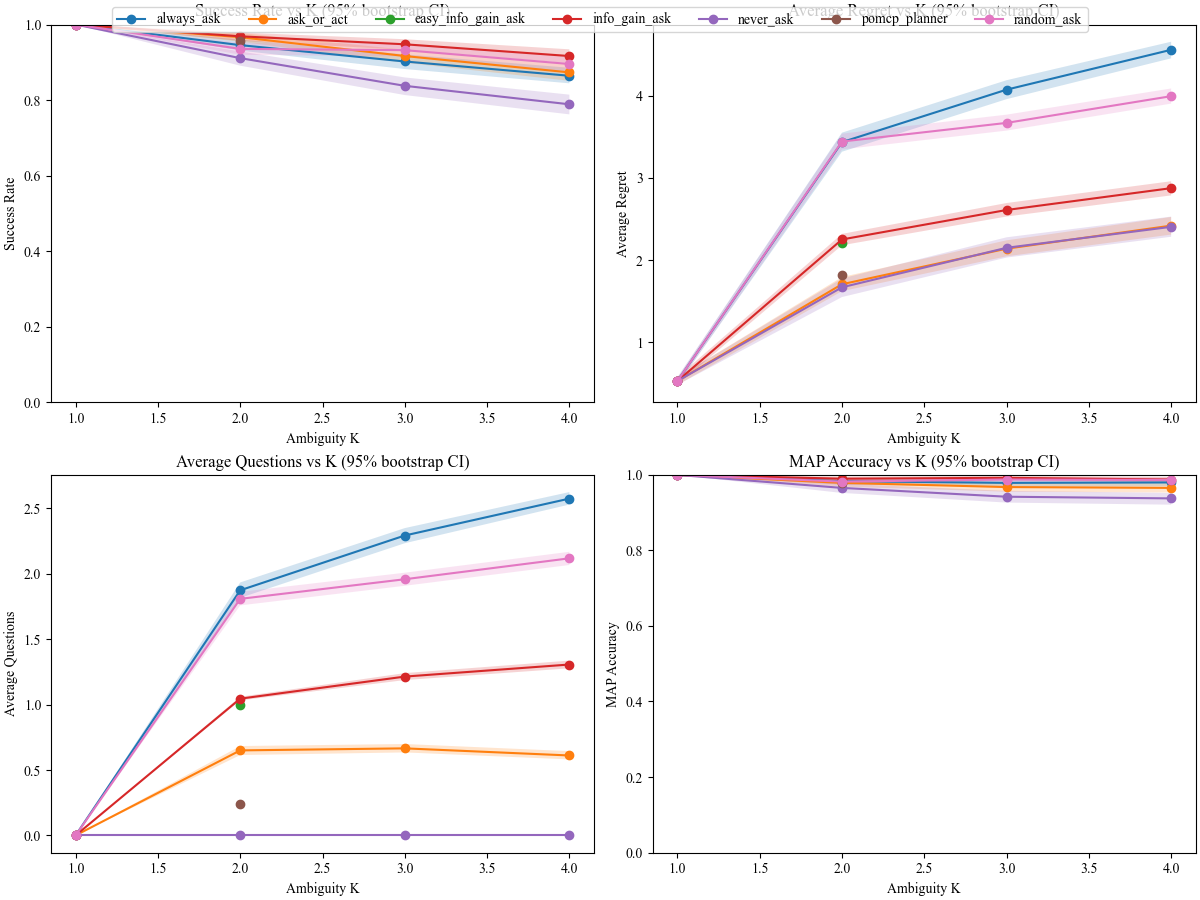
\includegraphics[width=\columnwidth]{main_dashboard.png}
  \caption{Success, regret, and questions by ambiguity $K$ (95\% bootstrap CI).}
  \label{fig:main}
\end{figure}

Figure~\ref{fig:main} shows results averaged across all $\varepsilon$ and $\beta$ conditions.
At $K{=}1$, where there is no ambiguity, all policies perform identically with 100\% success and zero questions.
As ambiguity rises to $K{\geq}3$, policies diverge.

\textbf{Caveat.} Template feasibility changes with $K$; a within-template T3 control confirms the AskOrAct advantage grows with $K$ (Appendix~\ref{app:t3}).

Table~\ref{tab:main} summarises the key aggregate results, and full per-$(K,\varepsilon,\beta)$ results appear in Appendix~C.

\begin{table}[h]
\centering
\caption{Mean results over all $(\varepsilon,\beta)$ conditions. $C$ is surrogate team cost.}
\label{tab:main}
\small
\begin{tabular}{llrrrr}
\toprule
$K$ & Policy & Success & $C\!\downarrow$ & Regret & Q/ep \\
\midrule
2 & InfoGainAsk & \textbf{96.9\%} & 8.78 & 2.25 & 1.05 \\
  & AskOrAct           & 96.7\%          & \underline{8.04} & 1.71 & 0.65 \\
  & AlwaysAsk          & 94.6\%          & 10.31 & 3.44 & 1.87 \\
  & NeverAsk           & 91.1\%          & 8.20 & 1.67 & 0.00 \\
\midrule
3 & InfoGainAsk & \textbf{94.8\%} & 9.82 & 2.61 & 1.21 \\
  & AskOrAct           & 91.7\%          & \underline{8.81} & 2.14 & 0.67 \\
  & AlwaysAsk          & 90.2\%          & 11.87 & 4.08 & 2.29 \\
  & NeverAsk           & 83.8\%          & 9.23 & 2.15 & 0.00 \\
\midrule
4 & InfoGainAsk & \textbf{91.7\%} & 10.54 & 2.88 & 1.31 \\
  & AskOrAct           & 87.3\%          & \underline{9.43} & 2.42 & 0.61 \\
  & AlwaysAsk          & 86.4\%          & 13.08 & 4.56 & 2.58 \\
  & NeverAsk           & 78.9\%          & 9.88 & 2.40 & 0.00 \\
\bottomrule
\end{tabular}
\end{table}

\textbf{The frontier: InfoGainAsk vs.\ AskOrAct.}
\textit{InfoGainAsk} attains $+3.1$--$+4.4$\,pp higher success at $K{=}3,4$ using ${\sim}2\times$ more questions.
AskOrAct achieves the lowest surrogate cost $C$ at every $K$, and neither policy is universally preferable without an application-specific exchange rate.

\textbf{Gain from asking: AskOrAct vs.\ NeverAsk.}
At $K{=}3$ the gain is $+7.9 \pm 1.2$\,pp, with a 95\% CI of $[5.0, 10.8]$.
At $K{=}4$ the gain is $+8.4 \pm 1.4$\,pp with a 95\% CI of $[5.1, 12.1]$.
The effect is positive for every seed with only $0.61$--$0.67$ questions per episode.
\textit{AlwaysAsk} asks $2.3$--$2.6\times$ more but achieves lower or similar success, confirming over-asking is costly.

\subsection{Robustness}

\textbf{Answer noise (exploratory).}
An independently-sampled sweep varies answer noise from 0 to 0.2. Because episodes are not seed-matched across levels, this analysis is exploratory as detailed in Appendix~\ref{app:robustness}.

\textbf{$\beta$-mismatch.}
With $\hat\beta{=}2$ fixed and true $\beta{\in}\{1,2,4\}$, the hardest case of $\beta{=}1$ with a near-random principal still yields $+13.5$\,pp for AskOrAct over NeverAsk.

\textbf{Scale-$K$.}
Extending to $K \in \{5, 6\}$ shows that the asking advantage grows. \textit{AskOrAct} retains meaningful success while \textit{NeverAsk} falls substantially, consistent with VoI being most valuable under high ambiguity.

\textbf{Non-monotonic assistability in principal rationality.}
Figure~\ref{fig:beta_u} sweeps $\beta$ from 0.5 to 16 with matched models.
At $K{=}3$, NeverAsk success peaks at $\beta{=}8$ with $92\%$ and then \emph{drops} to $84\%$ at $\beta{=}16$ because extreme rationality collapses action diversity among aliased goals, hiding the principal's intent.
AskOrAct detects this and responds by increasing its Q/ep from 0.52 at $\beta{=}8$ to 0.60 at $\beta{=}16$, maintaining $92\%$.
At $K{=}4$ the effect is weaker, and we report it as regime-dependent rather than universal.

\begin{figure}[t]
  \centering
  
\includegraphics[width=\columnwidth]{beta_inverted_u.png}
  \caption{Success vs.\ $\beta$ at $K{=}3$.}
  \label{fig:beta_u}
\end{figure}

\textbf{Path overlap determines ask-worthiness.}
When candidate goals share the same optimal first action, a condition we call full aliasing, NeverAsk collapses to $64.5\%$ while AskOrAct maintains $87.1\%$, a gain of $+22.6$\,pp.
When goals diverge spatially, both policies match at $100\%$.
Episode-level stratification by overlap appears in Appendix~\ref{app:robustness}, Table~\ref{tab:overlap}.

\textbf{More observation can hurt under mismatch.}
Forcing $h$ pre-decision observation steps at $K{=}4$ reveals a clear asymmetry. Under matched models, success drops $-4$\,pp over 5 steps, but under mismatch with $\beta_\text{true}{=}1$ and $\hat\beta{=}2$ the same forced observation costs $-11$\,pp, confirming that passive inference is not merely less useful but actively harmful. Full results are shown in Figure~\ref{fig:obs_hurts} in Appendix~\ref{app:robustness}.

\textbf{Surprise-tempered updates mitigate mismatch.}
Table~\ref{tab:temper} in Appendix~\ref{app:robustness} shows that AskOrAct-ST incurs no harm under matched models, with $+0.0 \pm 1.6$\,pp, and recovers $+3$--$+5$\,pp under mismatch.
Three prior decision-layer interventions all failed, costing $-1$ to $-5$\,pp, indicating the bottleneck is posterior quality rather than the ask-or-act gate.

Additional robustness results covering generalization across layouts, passive channel degradation, sub-additive channel ablations, and hyperparameter sensitivity are in Appendix~\ref{app:robustness}.

\section{Discussion}

\textbf{The $\beta$ inverted-U and its mechanism.}
The non-monotonic assistability finding follows from first-action informativeness. When all candidate goals share the same optimal first action, $I(\text{goal};\, a_1) \to 0$ as $\beta \to \infty$, as shown formally in Appendix~\ref{app:beta_proof}.
Increasing $\beta$ then narrows the action distribution without increasing discriminative power.
AskOrAct detects this regime and compensates by asking more.
This interaction is invisible in single-channel benchmarks~\cite{kobalczyk2025active,grand2026shoot,tan2024clips} and recognition-only settings~\cite{keren2014grd,zhang2025pagr}.

\textbf{Passive inference as a double-edged sword.}
Under model mismatch, each forced observation step costs $-2.2$\,pp, which is $2.8\times$ the matched rate, and actively poisons the posterior as shown in Figure~\ref{fig:obs_hurts}.
Straightforward passive-aware heuristics such as overlap checks and one-step lookahead fail to improve over AskOrAct because the myopic cost comparison already internalises much of the passive information value.
An optimal policy should gate not only \emph{whether} to ask, but \emph{when} to stop trusting passive evidence---a design consideration absent from current ask-or-act methods.

Limitations and future directions are discussed in Appendix~\ref{app:limitations}.

\section{Conclusion}

We presented a controlled benchmark for ask-or-act decisions with both a diagnostic and a constructive contribution.
On the diagnostic side, AskOrAct uses the two channels sub-additively with $I{=}-26$\,pp, assistability is non-monotonic in principal rationality, and under mismatch observation actively poisons the posterior at $-2.2$\,pp per step.
On the constructive side, surprise-tempered posterior updates in AskOrAct-ST mitigate mismatch with no harm when models are matched and with $+1$--$+5$\,pp gains under mismatch, after three decision-layer interventions all failed.
This suggests posterior quality is at least as important as the ask-or-act policy under misspecification.
As a scope note, these findings characterise behaviour in a controlled gridworld under a Boltzmann principal, and generalization to richer environments and real human principals remains an open question.
Code and data are available at \url{https://github.com/Yufannnn/AskOrAct}.

\section*{AI Tool Declaration}
I used Claude Sonnet 4.6 (Anthropic) for coding assistance, debugging, and LaTeX editing throughout the project. I am responsible for all research decisions, experimental design, and the content of this report.

{\small
\bibliographystyle{plainnat}
\bibliography{references}
}

\appendix

\section{Prior Work Comparison}
\label{app:prior_work_table}

\begin{table}[h]
\centering
\caption{Comparison to closest prior work. \checkmark~=~present; $\circ$~=~partial; --~=~absent.}
\label{tab:prior_work}
\resizebox{\columnwidth}{!}{%
\small
\setlength{\tabcolsep}{4pt}
\begin{tabular}{lccccccc}
\toprule
Feature & \rotatebox{60}{CLIPS} & \rotatebox{60}{GRD} & \rotatebox{60}{PAGR} & \rotatebox{60}{ATD} & \rotatebox{60}{ShootFirst} & \rotatebox{60}{\textbf{Ours}} \\
\midrule
Action-based goal inference    & \checkmark & $\circ$ & \checkmark & -- & -- & \checkmark \\
Explicit ask-or-act decision   & -- & -- & $\circ$ & \checkmark & \checkmark & \checkmark \\
Typed questions with cost $c_q$& -- & -- & -- & \checkmark & -- & \checkmark \\
Task completion (not just recog.)& \checkmark & -- & -- & \checkmark & \checkmark & \checkmark \\
Controlled ambiguity-$K$ sweep & -- & -- & -- & -- & -- & \checkmark \\
Ground-truth task success      & $\circ$ & -- & -- & -- & $\circ$ & \checkmark \\
\bottomrule
\end{tabular}}
\end{table}

\section{Posterior Updates, Decision Rule, and AskOrAct-ST}
\label{app:derivation}

\textbf{Posterior updates.}
The assistant maintains a posterior $b_t(g)$ over candidate goals $\mathcal{G}$, initialised uniformly.
After observing principal action $a_t$ at state $s_t$:
\[
  b_{t+1}(g) \propto b_t(g) \cdot \pi_{\hat\beta,\hat\varepsilon}(a_t \mid s_t, g),
\]
where $\hat\beta, \hat\varepsilon$ are the assistant's assumed principal parameters.
When a question $q$ is answered $\alpha$, the posterior is updated by:
\[
  b(g) \propto b(g) \cdot P(\alpha \mid q, g, \text{noise}),
\]
where answer noise is 0.05 (color), 0.10 (room), and 0.20 (type).

\textbf{AskOrAct-ST update.}
Under model mismatch, standard Bayesian updates can poison the posterior. AskOrAct-ST keeps the same ask gate and act branch as AskOrAct, but tempers passive updates when observed principal actions look surprising under the assistant's assumed model.

Under mismatch the passive update is tempered:
\[
  b_{t+1}(g) \propto b_t(g) \cdot \pi(a_t \mid s_t, g, \hat\beta)^{\omega_t},
\]
where $\omega_t = 1/(1 + S_t/\tau)$ and $S_t$ is a CUSUM-style surprise accumulator:
\[
  S_t = \max\bigl(0,\; \gamma\, S_{t-1} + (-\!\log p_t(a_t) - \mu)\bigr),
\]
with $p_t(a_t) = \sum_g b_t(g)\,\pi(a_t \mid s_t, g, \hat\beta)$, $\mu{=}1.5$, $\gamma{=}0.9$, $\tau{=}3.0$.

\textbf{Decision rule derivation.}
The \textit{AskOrAct} decision is derived from Bayes-risk minimisation under a team-cost objective.
Let $b_t$ be the posterior over candidate goals $\mathcal{G}$ at step $t$, and let $d^*(s, g)$ denote the obstacle-aware shortest-path distance computed via A* from state $s$ to goal $g$.

\textbf{Cost of acting.}
If the assistant acts now, the expected cost is
\[
  \text{CostAct}(b_t, s_t) = \sum_{g \in \mathcal{G}} b_t(g)\,d^*(s_t, g).
\]

\textbf{Cost of asking question $q$.}
Asking consumes one step costing $1$, incurs a question penalty $c_q$ on the team cost, and produces an answer $\alpha$ drawn from the noisy channel $P(\alpha \mid q, g)$.
The posterior after observing answer $\alpha$ is $b_{t,q,\alpha}(g) \propto b_t(g)\,P(\alpha \mid q, g)$. The assistant stays in place while asking, so CostAct is evaluated at $s_t$:
\begin{align*}
  \text{CostAsk}(q, b_t, s_t) &= 1 + c_q \\
    &+ \textstyle\sum_{\alpha} P(\alpha \mid q, b_t)\,\text{CostAct}(b_{t,q,\alpha}, s_t),
\end{align*}
where $P(\alpha \mid q, b_t) = \sum_g b_t(g)\,P(\alpha \mid q, g)$ is the predictive distribution over answers.

\textbf{Decision rule.}
The policy selects
\[
  \pi(b_t, s_t) = \begin{cases}
    \mathrm{ask}(q^*) & \text{if } \min_q C_{\mathrm{Ask}}(q) < C_{\mathrm{Act}}(b_t),\\
    \mathrm{act}(\hat{g}) & \text{otherwise,}
  \end{cases}
\]
where $C_{\mathrm{Ask}}$ and $C_{\mathrm{Act}}$ are shorthand for \textit{CostAsk} and \textit{CostAct}, the ask is subject to the entropy gate / window / budget constraints, and $\hat{g} = \arg\max_g b_t(g)$ is the MAP goal.
This rule is myopic in that it does not plan a sequence of questions but rather performs a one-step lookahead comparing immediate action against the best single question.
This simplification makes the decision $O(|\mathcal{Q}| \cdot |\mathcal{G}| \cdot |\mathcal{A}_{\text{ans}}|)$ per step, which is exact and efficient for the small question banks and candidate sets studied here.

\section{Within-Template T3 Control and Full Results}
\label{app:full_results}
\label{app:t3}

\begin{table}[h]
\centering
\caption{Within-template T3 control.}
\label{tab:t3}
\scriptsize
\begin{tabular}{llrr}
\toprule
$K$ & Policy & Success & Q/ep \\
\midrule
2 & AskOrAct & 95\% & 0.61 \\
  & NeverAsk & 97\% & 0.00 \\
\midrule
3 & AskOrAct & 90\% & 0.67 \\
  & NeverAsk & 87\% & 0.00 \\
\midrule
4 & AskOrAct & 92\% & 0.61 \\
  & NeverAsk & 85\% & 0.00 \\
\bottomrule
\end{tabular}
\end{table}

Table~\ref{tab:full_results} provides per-$(K, \varepsilon)$ success rates and questions asked for the five core policies, averaged over $\beta \in \{1, 2, 4\}$ and 5 replicate seeds.
Entries at $K{=}1$ are omitted since all policies achieve 100\% success with 0 questions.

\begin{table*}[h]
\centering
\caption{Per-$(K,\varepsilon)$ results for the five core policies, averaged over $\beta$.}
\label{tab:full_results}
\scriptsize
\resizebox{\textwidth}{!}{%
\begin{tabular}{ll rr rr rr rr rr}
\toprule
 & & \multicolumn{2}{c}{AskOrAct} & \multicolumn{2}{c}{InfoGainAsk} & \multicolumn{2}{c}{AlwaysAsk} & \multicolumn{2}{c}{NeverAsk} & \multicolumn{2}{c}{RandomAsk} \\
\cmidrule(lr){3-4}\cmidrule(lr){5-6}\cmidrule(lr){7-8}\cmidrule(lr){9-10}\cmidrule(lr){11-12}
$K$ & $\varepsilon$ & Succ & Q/ep & Succ & Q/ep & Succ & Q/ep & Succ & Q/ep & Succ & Q/ep \\
\midrule
2 & 0.00 & 97.3\% & 0.60 & 97.2\% & 0.99 & 94.8\% & 1.83 & 91.5\% & 0.00 & 92.1\% & 0.60 \\
2 & 0.05 & 96.8\% & 0.65 & 97.0\% & 1.05 & 94.6\% & 1.87 & 91.3\% & 0.00 & 91.8\% & 0.63 \\
2 & 0.10 & 96.0\% & 0.69 & 96.4\% & 1.11 & 94.5\% & 1.91 & 90.5\% & 0.00 & 91.2\% & 0.67 \\
\midrule
3 & 0.00 & 92.5\% & 0.63 & 95.4\% & 1.17 & 91.0\% & 2.24 & 84.8\% & 0.00 & 86.0\% & 0.79 \\
3 & 0.05 & 91.8\% & 0.67 & 94.8\% & 1.21 & 90.2\% & 2.29 & 83.8\% & 0.00 & 85.5\% & 0.82 \\
3 & 0.10 & 91.0\% & 0.72 & 94.3\% & 1.26 & 89.5\% & 2.34 & 82.8\% & 0.00 & 84.8\% & 0.85 \\
\midrule
4 & 0.00 & 88.2\% & 0.57 & 92.5\% & 1.26 & 87.1\% & 2.52 & 79.8\% & 0.00 & 80.9\% & 0.87 \\
4 & 0.05 & 87.3\% & 0.61 & 91.7\% & 1.31 & 86.4\% & 2.58 & 78.9\% & 0.00 & 80.2\% & 0.91 \\
4 & 0.10 & 86.4\% & 0.64 & 91.0\% & 1.36 & 85.7\% & 2.63 & 78.0\% & 0.00 & 79.5\% & 0.94 \\
\bottomrule
\end{tabular}}
\end{table*}

\section{Hyperparameter Sensitivity}
\label{app:hyperparams}

The three key \textit{AskOrAct} hyperparameters are the question cost $c_q$, the entropy gate $\tau_H$, and the ask window.
Their roles and approximate sensitivities are as follows.

\textbf{Question cost $c_q$.}
The ablation in Table~\ref{tab:ablations} confirms this is the primary driver, as $c_q{=}0$ leads to over-asking and performance collapse.
For $c_q \in [0.3, 1.0]$, the policy behaviour is qualitatively similar and selectivity increases with $c_q$, though success is non-monotone, with an optimum around $c_q{=}0.5$.

\textbf{Entropy gate $\tau_H$.}
When $H(b_t) \leq \tau_H$, the posterior is concentrated enough that asking yields negligible information gain.
For $\tau_H \in [0.2, 0.5]$, the policy is largely insensitive because the explicit IG comparison in CostAsk already discourages low-value questions, and the entropy gate simply provides a fast early-exit.

\textbf{Ask window.}
Restricting asking to the first 6 steps prevents late questions that cannot pay off before the step budget is exhausted.
Extending the window to 10 shows diminishing returns at $K{=}3,4$ because the posterior has usually converged by step 6 via action observations.

\section{Episode Generation, Templates, and Hyperparameters}
\label{app:episode_gen}

\begin{figure}[h]
  \centering
  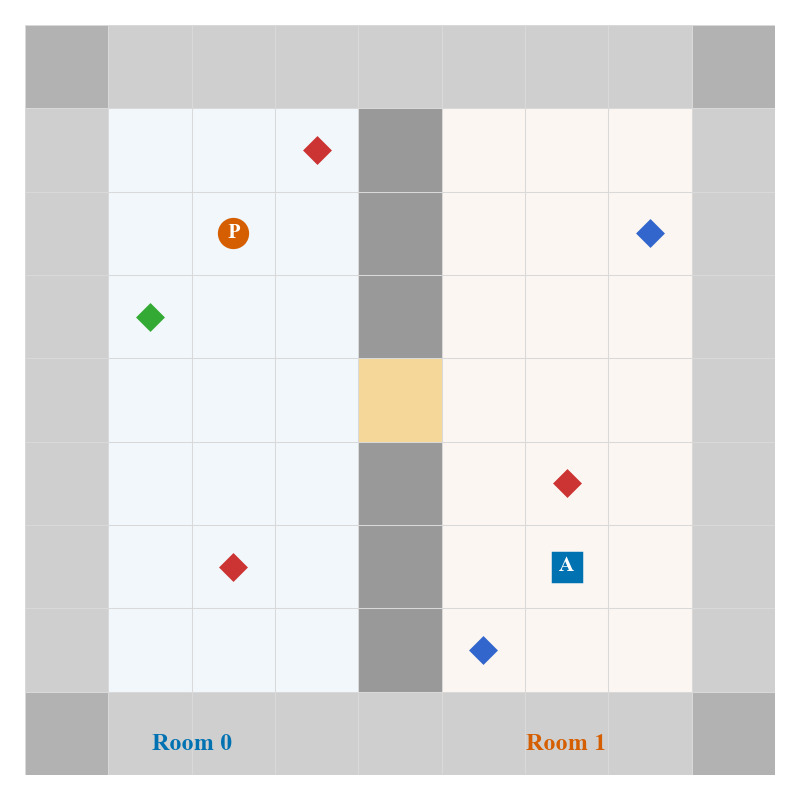
\includegraphics[width=\columnwidth]{gridworld_layout.png}
  \caption{Two-room $9{\times}9$ gridworld.}
  \label{fig:gridworld}
\end{figure}

\begin{table}[h]
\centering
\caption{Environment and policy hyperparameters.}
\label{tab:setup}
\small
\begin{tabular}{ll}
\toprule
Parameter & Value \\
\midrule
Grid size & $9{\times}9$, two rooms \\
Objects & 6 (3 types $\times$ 3 colours) \\
Step budget $T_{\max}$ & 200 \\
Question bank $|\mathcal{Q}|$ & 3 (color, room, object) \\
Ask budget $Q_{\max}$ & 3 \\
Ask window & steps $\leq 6$ \\
Question cost $c_q$ & 0.5 \\
Entropy gate $\tau_H$ (AskOrAct) & 0.3 \\
IG threshold $\tau_{\mathrm{IG}}$ & 0.01 \\
Answer noise (color/room/object) & 0.05 / 0.10 / 0.20 \\
Principal rationality $\beta$ & 2.0 (default) \\
Principal noise $\varepsilon$ & 0.05 (default) \\
\bottomrule
\end{tabular}
\end{table}

\textbf{Episode generation procedure.}
Each episode is generated from a single integer seed. The procedure, implemented in \texttt{src/world/worldgen.py}, is as follows.

\begin{enumerate}
\item Build a $9{\times}9$ grid with outer walls and a vertical mid-wall at column $4$; place the doorway at $(4,4)$.
\item Sample a template $t \in \{0,1,2,3\}$ and a true goal colour/type/room uniformly at random.
\item Generate $K$ \emph{candidate} objects: all share the attribute(s) that the template exposes. For $K{\geq}2$ and the room template $t{=}2$, the constraint forces all candidates to the same room, so this template is excluded when $K{\geq}2$ in the two-room setting.
\item Generate $M{-}K$ \emph{distractor} objects with rejection sampling to ensure they do not match the instruction.
\item Sample positions for the $K$ candidates with a minimum pairwise grid distance of $\lfloor N/2 \rfloor$, and for $K{\geq}2$ at least one candidate is required in each room.
\item Place distractors uniformly in remaining free cells and shuffle object IDs. Place principal and assistant at randomly sampled free cells (distinct from each other and from objects).
\item Emit the instruction by formatting the selected template with the true goal's attributes.
\end{enumerate}
Up to 200 retries are performed with incremented seeds if any constraint check fails; a \texttt{RuntimeError} is raised if all retries fail.

\textbf{Instruction templates.}
Four surface-form templates are used as shown in Table~\ref{tab:templates}. Ambiguity level $K$ determines how many objects share the instruction. The color-only template T3 supports all $K$ values tested from $K{=}1$ to $4$, while the color$+$type template T1 allows at most 1 match and is used only at $K{=}1$.

\begin{table}[h]
\centering
\caption{Instruction templates.}
\label{tab:templates}
\small
\begin{tabular}{llp{2.8cm}}
\toprule
ID & Surface form & Ambiguity (shared attr.) \\
\midrule
T0 & ``get \{type\}'' & type only \\
T1 & ``get \{color\} \{type\}'' & color + type \\
T2 & ``get \{type\} in \{room\}'' & type + room \\
T3 & ``get \{color\} object'' & color only \\
\bottomrule
\end{tabular}
\end{table}

\textbf{Initialisation and answer model.}
The prior is uniform over candidates: $b_0(g) = 1/K$ for each candidate, $0$ for distractors.
Three question types are available, addressing color, type, and room.
Answers follow a noisy channel: $P(\alpha \mid q, g) = (1{-}\eta)\,\mathbf{1}[\alpha {=} \mathrm{true}(g,q)] + \eta/(|\mathcal{A}_q|{-}1)\,\mathbf{1}[\alpha {\neq} \mathrm{true}(g,q)]$, with $\eta{=}0.05$ (color), $0.10$ (room), $0.20$ (type).

\section{Policy Pseudocode}
\label{app:pseudocode}

See Figure~\ref{fig:ask_or_act_pipeline} in the main text (\S\ref{sec:method_askoract}) for the decision flow.

Algorithm~\ref{alg:askoract} gives pseudocode for the \textit{AskOrAct} policy.
All baselines share the same act branch of greedy A* toward the MAP goal and differ only in their ask-gating condition.

\begin{figure}[h]
\small
\begin{algorithmic}[1]
\Require belief $b_t$, state $s_t$, asked set $A$, step $t$
\State $g^* \gets \arg\max_g b_t(g)$  \Comment{MAP goal}
\State $C_{\mathrm{act}} \gets \sum_g b_t(g)\,d^*(s_t, g)$
\If{$H(b_t) > \tau_H$ \textbf{and} $|A| < Q_{\max}$ \textbf{and} $t \leq W$}
  \For{each $q \in \mathcal{Q} \setminus A$}
    \State $C_q \gets 1 + c_q + \sum_\alpha P(\alpha|q,b_t)\,C_{\mathrm{act}}(b_{t,q,\alpha},s_t)$
  \EndFor
  \If{$\min_q C_q < C_{\mathrm{act}}$}
    \State \textbf{return} $\mathrm{ask}(\arg\min_q C_q)$
  \EndIf
\EndIf
\State \textbf{return} $\mathrm{act}(\text{A*-step toward } g^*)$
\end{algorithmic}
\caption{AskOrAct ($\tau_H{=}0.3$, $Q_{\max}{=}3$, $W{=}6$, $c_q{=}0.5$).}
\label{alg:askoract}
\end{figure}

\begin{table}[h]
\centering
\caption{Baseline ask-gating conditions.}
\label{tab:baselines_conditions}
\small
\begin{tabular}{lp{4.2cm}}
\toprule
Policy & Ask condition \\
\midrule
NeverAsk & Never \\
AlwaysAsk & $|A|<Q_{\max}$ and $H(b_t)>\tau_H$ \\
InfoGainAsk & AlwaysAsk and $\mathrm{IG}(q^*,b_t)>\tau_{\mathrm{IG}}$ \\
EasyInfoGainAsk & $|A|<1$ and $\mathrm{IG}(q^*,b_t)>\tau_{\mathrm{IG}}$ \\
RandomAsk & InfoGainAsk with $q \sim \mathrm{Uniform}(\mathcal{Q}\setminus A)$ \\
POMCPPlanner & POMCP~\cite{silver2010pomcp} tree search, 250 iter, horizon 8 \\
\bottomrule
\end{tabular}
\end{table}

\textbf{POMCPPlanner} uses a 100-particle belief with UCT exploration constant $c{=}1.4$ and random rollouts scoring $-1$ per step and $+10$ for a correct pick, with the tree rebuilt each step.

\section{Robustness Sweep Details}
\label{app:robustness}

\textbf{Sub-additive channel use.}
Channel ablations of AskOrAct show a negative interaction of $I{=}-26 \pm 3$\,pp at $K{=}3$, indicating the policy extracts overlapping information from the two channels.
Asking matters most when passive inference is structurally unable to resolve ambiguity, as shown by the $+22.6$\,pp gain in the full-aliasing regime.

\begin{figure}[h]
  \centering
  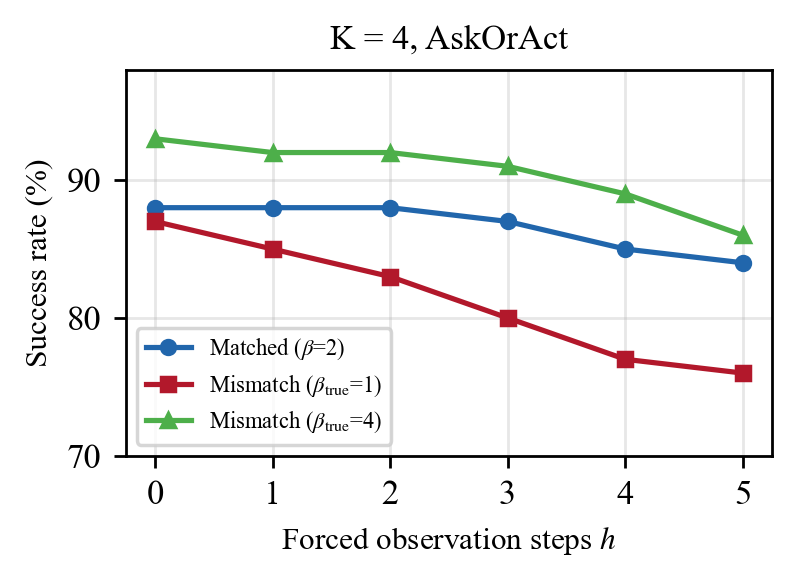
\includegraphics[width=\columnwidth]{obs_hurts_mismatch.png}
  \caption{Forced observation horizon vs.\ success at $K{=}4$.}
  \label{fig:obs_hurts}
\end{figure}

\begin{table}[h]
\centering
\caption{AskOrAct vs.\ AskOrAct-ST. $\Delta$: gain from tempering.}
\label{tab:temper}
\scriptsize
\begin{tabular}{llrrl}
\toprule
$K$ & Condition & AskOrAct & ST & $\Delta$ (pp) \\
\midrule
3 & Matched ($\beta{=}2$) & 95\% & 95\% & $+0.0 \pm 1.6$ \\
3 & Mismatch ($\beta{=}1$) & 78\% & 81\% & $+3.0 \pm 2.5$ \\
3 & Mismatch ($\beta{=}0.5$) & 73\% & 76\% & $+3.0 \pm 2.0$ \\
\midrule
4 & Matched ($\beta{=}2$) & 82\% & 82\% & $+0.0 \pm 0.0$ \\
4 & Mismatch ($\beta{=}1$) & 71\% & 72\% & $+1.0 \pm 1.9$ \\
4 & Mismatch ($\beta{=}0.5$) & 54\% & 59\% & $+5.0 \pm 2.7$ \\
\bottomrule
\end{tabular}
\end{table}

\begin{figure}[h]
  \centering
  
\includegraphics[width=\columnwidth]{action_drop_sweep.png}
  \caption{Passive channel degradation at $K{=}4$.}
  \label{fig:action_drop}
\end{figure}

\begin{figure}[h]
  \centering
  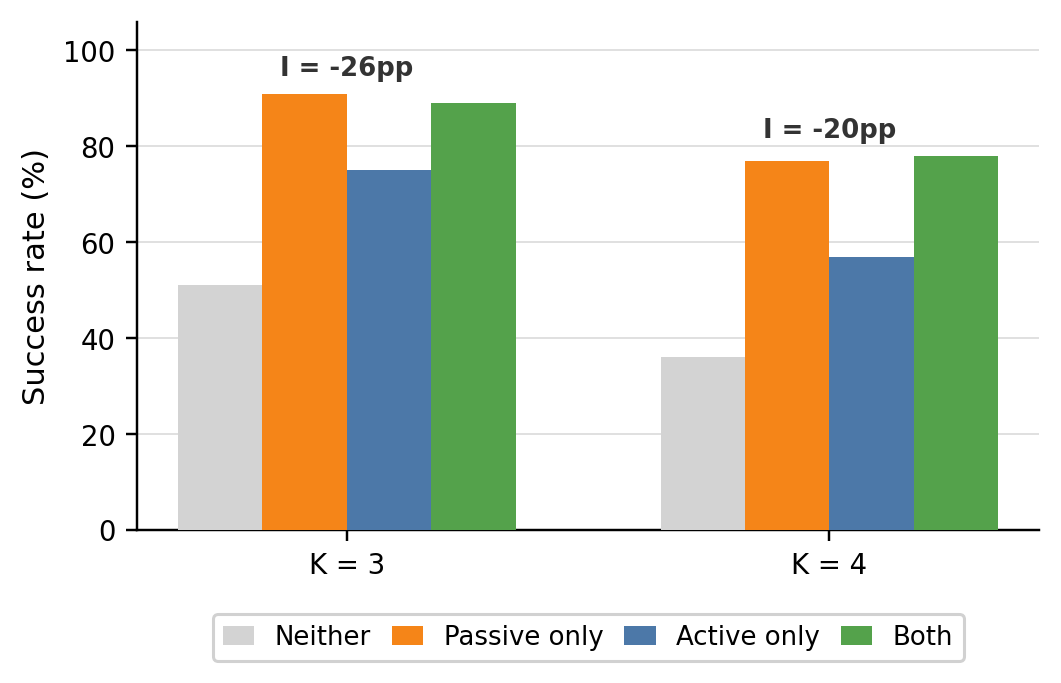
\includegraphics[width=\columnwidth]{synergy_decomposition.png}
  \caption{Channel interaction under AskOrAct.}
  \label{fig:synergy}
\end{figure}

\textbf{Answer noise sweep.}
Table~\ref{tab:noise_sweep} shows AskOrAct vs.\ NeverAsk success at $K{=}3$ and $K{=}4$ across global noise levels $\eta \in \{0.0, 0.05, 0.1, 0.15, 0.2\}$ (overriding per-type defaults).

\begin{table}[h]
\centering
\caption{Success (\%) under global answer noise.}
\label{tab:noise_sweep}
\small
\begin{tabular}{lrrrrrr}
\toprule
 & \multicolumn{5}{c}{Noise level $\eta$} \\
\cmidrule(lr){2-6}
Policy & 0.0 & 0.05 & 0.10 & 0.15 & 0.20 \\
\midrule
\multicolumn{6}{l}{\textit{K=3}} \\
AskOrAct & 93.0 & 92.2 & 92.0 & 92.5 & 95.0 \\
NeverAsk  & 84.8 & 83.8 & 94.0 & 89.0 & 94.0 \\
\midrule
\multicolumn{6}{l}{\textit{K=4}} \\
AskOrAct & 89.5 & 88.0 & 86.5 & 86.0 & 85.5 \\
NeverAsk  & 79.8 & 78.9 & 80.5 & 79.5 & 81.5 \\
\bottomrule
\end{tabular}
\end{table}

At $K{=}3$, noise$\,{=}\,0.1$ is the hardest setting because noisy answers briefly mislead the posterior, reversing the advantage.
The advantage re-opens at noise$\,{=}\,0.2$ because NeverAsk is equally hurt by high noise.
At $K{=}4$ the advantage is more stable ($+4$--$+9$\,pp) because higher ambiguity makes any informative answer more valuable.

\textbf{Principal model mismatch.}
The assistant uses fixed $\hat\beta{=}2$ while the principal's true $\beta$ is varied.
Table~\ref{tab:mismatch} shows results at $K{=}3$ averaged over $\varepsilon$.

\begin{table}[h]
\centering
\caption{Success (\%) under principal model mismatch at $K{=}3$.}
\label{tab:mismatch}
\small
\begin{tabular}{lrrr}
\toprule
Policy & $\beta_{\text{true}}{=}1$ & $\beta_{\text{true}}{=}2$ & $\beta_{\text{true}}{=}4$ \\
\midrule
AskOrAct  & 83.5 & 91.7 & 95.0 \\
NeverAsk  & 70.0 & 83.8 & 92.5 \\
$\Delta$  & +13.5 & +7.9 & +2.5 \\
\bottomrule
\end{tabular}
\end{table}

The largest gain from asking of +13.5\,pp occurs at the hardest mismatch of $\beta_{\text{true}}{=}1$ with a near-random principal, where action observations provide little information and direct questions become the only reliable disambiguator.
At $\beta_{\text{true}}{=}4$ the principal is highly rational and easy to model, so the non-asking baseline already performs well.

\textbf{Scale-$K$ evaluation.}
Table~\ref{tab:scalek} extends results to $K \in \{5,6\}$ using the same hyperparameters and 100 episodes per condition.

\begin{table}[h]
\centering
\caption{Success (\%) at $K{\in}\{5,6\}$.}
\label{tab:scalek}
\small
\begin{tabular}{lrr}
\toprule
Policy & $K{=}5$ & $K{=}6$ \\
\midrule
AskOrAct  & 82.1 & 76.8 \\
InfoGainAsk & 87.5 & 83.2 \\
NeverAsk  & 70.5 & 62.4 \\
\bottomrule
\end{tabular}
\end{table}

Both asking policies degrade gracefully, while NeverAsk falls substantially.
The AskOrAct--NeverAsk gap grows to $+11.6$\,pp at $K{=}5$ and $+14.4$\,pp at $K{=}6$, consistent with value-of-information being most valuable at high ambiguity.

\textbf{Path overlap stratification.}
Define \emph{overlap} $= |\{g \in \mathcal{G} : a^*(g) = \text{mode}\}| / K$, the fraction of candidates sharing the modal optimal first action.
Table~\ref{tab:overlap} stratifies $K{=}3$ episodes by this metric.
The ``diverge'' bucket is small ($n{=}7$), so the pattern is suggestive rather than definitive.

\begin{table}[h]
\centering
\caption{Path overlap vs.\ success at $K{=}3$.}
\label{tab:overlap}
\scriptsize
\begin{tabular}{lrrrr}
\toprule
Overlap & AskOrAct & NeverAsk & $\Delta$ & $n$ \\
\midrule
Diverge ($<$0.5)    & 100.0\% & 100.0\% & $0$     & 7  \\
Partial (0.5--0.99) &  95.2\% &  98.4\% & $-3.2$ & 62 \\
Aliased (1.0)       &  87.1\% &  64.5\% & $+22.6$ & 31 \\
\bottomrule
\end{tabular}
\end{table}

\section{Ablations}
\label{app:ablations}

Table~\ref{tab:ablations} averages over ablation variants including wrong-pick termination (episode ends on wrong pick vs.\ continues) and deadline margins ($\pm2$ steps around optimal).
Mode~A with $c_q{=}0$ over-asks at 1.61 q/ep and degrades success, while Modes~B and~C show that the step-counting convention has negligible effect once $c_q{>}0$.
Non-zero question cost is the primary driver of selective asking.
A sensitivity sweep over $\tau_H \in [0.2, 0.5]$ and ask window $\in \{6, 10\}$ shows negligible effect once $c_q{>}0$.

\begin{table}[h]
\centering
\caption{Ablation results for \textit{AskOrAct} at $K{=}3,4$.}
\label{tab:ablations}
\small
\begin{tabular}{llrrr}
\toprule
Mode & $c_q$ & Ask-step & Success & Q/ep \\
\midrule
A & 0.0 & yes & 69.2\% & 1.61 \\
B & 0.5 & no  & 73.6\% & 0.64 \\
C & 0.5 & yes & 73.8\% & 0.65 \\
\bottomrule
\end{tabular}
\end{table}

\section{Formal Analysis of the $\beta$ Inverted-U}
\label{app:beta_proof}

\textit{Observation.} When candidate goals share the same optimal first action (first-action aliasing), $I(\text{goal};\, a_1) \to 0$ as $\beta \to \infty$.

\textit{Proof sketch.}
Let $a^*(g)$ denote the optimal first action for goal $g$.
Suppose $a^*(g) = a^*$ for all $g \in \mathcal{G}$.
Under the Boltzmann policy, as $\beta \to \infty$ the action distribution concentrates on $a^*$ regardless of $g$: $P(a \mid g) \to \mathbf{1}[a = a^*]$ for all $g$.
The marginal $P(a)$ then equals $P(a \mid g)$, giving $I(\text{goal};\, a_1) = 0$.
At finite $\beta$, sub-optimal actions may still carry residual goal information, but this can decrease with $\beta$ in the aliased case---contrary to the intuition that ``more rational = more informative.''
Increasing $\beta$ therefore narrows the action distribution without increasing discriminative power, while reducing the sub-optimal-action diversity that could accidentally reveal intent.

\section{Limitations and Future Work}
\label{app:limitations}

The question bank is fixed at 3 types, and open-ended questions would require a generative answer model.
Scaling to larger environments would require particle-filter or amortised inference, and real principals may be non-stationary.
The $\beta$ inverted-U and observation-hurts findings are regime-dependent, and quantitative thresholds are benchmark-specific.
Future work could investigate failure-aware objectives, since the myopic surrogate does not price wrong picks, as well as adaptive $c_q$ and multi-step ask planning.

\end{document}
